\documentclass{article}
\usepackage[utf8]{inputenc}
\usepackage{amssymb}
\usepackage{relsize}
\usepackage{lscape}
\usepackage{graphicx}
\usepackage[bottom=0.6in,top=0.8in]{geometry}
\renewcommand*\familydefault{\sfdefault} %% Only if the base font of the document is to be sans serif
\usepackage{enumitem}
\usepackage[spanish]{babel} % Language hyphenation and typographical rules
\usepackage{hyperref}

\title{P4 BDD}
\author{merecmoney1 }
\date{March 2020}
\graphicspath{images/}

\begin{document}
    \begin{titlepage}
        \begin{center}
            {\bfseries\LARGE National Autonomous University of Mexico\par}
            \vspace{1cm}
            {\Large Faculty of Engineering \par}
            \vspace{1cm}
            {\LARGE Relational Distributed Databases \par}
            \vspace{3cm}
            {\Huge Practice 4\par}
            {\Huge Design of the Fragmentation Scheme \par}
            \vspace{1cm}
            {\Large Student: \par}
            {\Large Arrieta Carlos Alberto \par}
            {\Large Teacher: \par}
            {\Large Jorge Rodríguez Campos \par}
            {\Large Semester 2020-2 \par}
            {\Large March 5, 2020 \par} 
            \vspace{1cm}
            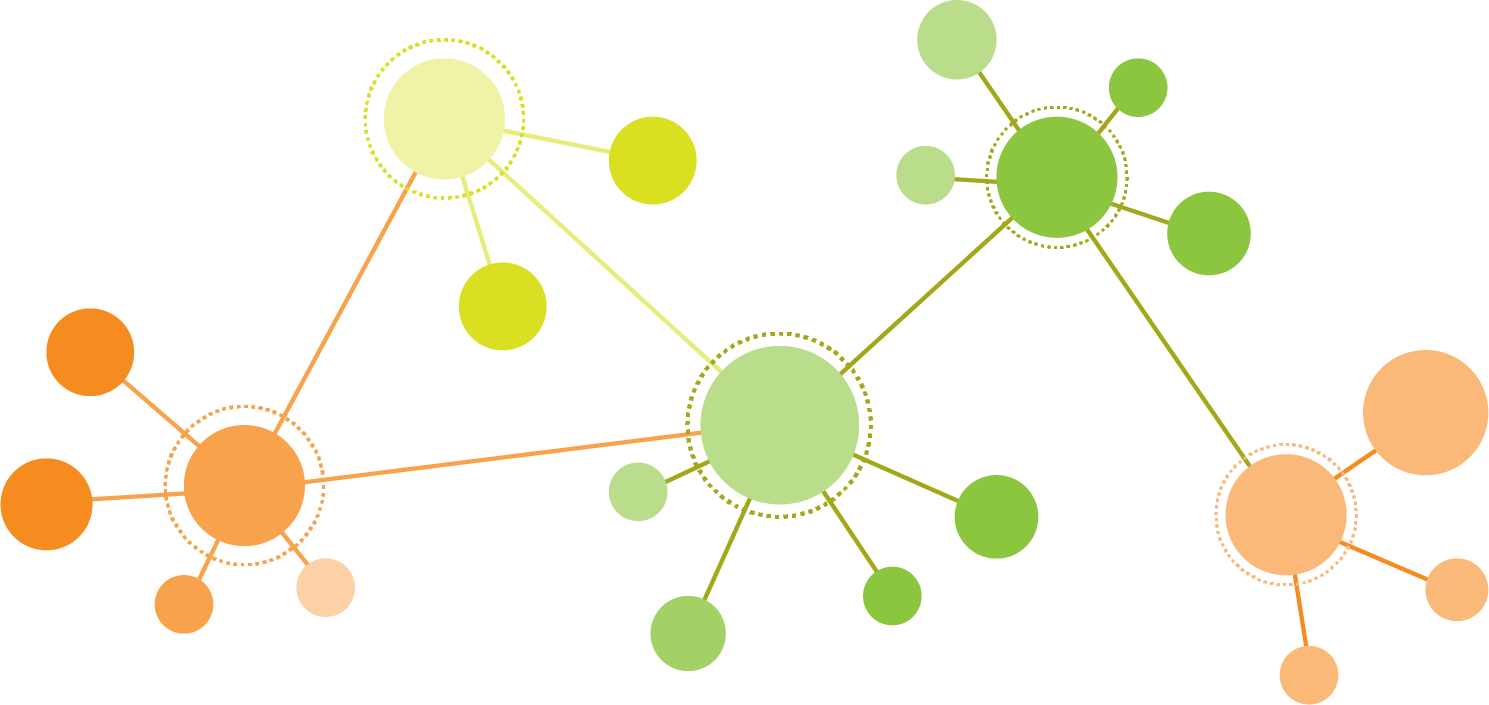
\includegraphics[scale=0.25]{images/graph_network.png}
        \end{center}

    \end{titlepage}
        

    \newpage
    
    \section{Objetivos}
    \begin{itemize}
          \item Poner en práctica los conceptos de fragmentación y sus diversos tipos a través de su implementación en un ambiente distribuido de 2 nodos.
          \item Experimentar técnicas para realizar la inserción y consulta de datos considerando un esquema de fragmentación sin aplicar aun los diferentes tipos de transparencia ni procesos o análisis de optimización.
    \end{itemize}

    \section{Introducción}
En esta práctica vamos a hacer uso de los conceptos vistos en clase para el diseño de una base de datos distribuida, sobre todo será énfasis en las estrategias de fragmentación, ya que teniendo las reglas de negocio debemos decidir si se  utiliza fragmentación horizontal (Primaria o Derivada), vertical o hibrida (horizontal y vertical). Haciendo uso de álgebra relacional se definirá las expresiones para fragmentar y reconstruir cada tabla en el caso de estudio, decidir en qué sitios vamos a colocar cada fragmento y crear un modelo relacional haciendo uso de la notación Crow’s Foot. Para el esquema relacional debemos analizar minuciosamente que restricciones de referencia vamos a conservar y eliminar.
    
    \begin{landscape}
    \section{Convenciones para el nombrado de fragmentos}
        \begin{tabular}{| c | c | p{1.5cm} |}
            \hline
            Fragment Name  & Expression of the Fragment & Fragment Location(N1 o N2) \\
            \hline
            \hline
            F\_CAH\_BANCO\_1 & $\sigma_{SUBSTR(CLAVE,1,1)\,BETWEEN\,'A'\,and\,'M'\,}(BANCO)$ & N1\\
            \hline
            F\_CAH\_BANCO\_2 & $\sigma_{SUBSTR(CLAVE,1,1)\,BETWEEN\,'N'\,and\,'Z'\,}(BANCO)$ & N2\\
            \hline                
            F\_CAH\_PAIS\_1 & $\sigma_{ZONA\_ECONOMICA = 'A'}(PAIS)$ & N1\\
            \hline
            F\_CAH\_PAIS\_2 & $\sigma_{ZONA\_ECONOMICA = 'B'}(PAIS)$ & N2\\
            \hline
            F\_CAH\_SUCURSAL\_1 & $SUCURSAL \ltimes_{BANCO\_ID} F\_CAH\_BANCO\_1$ & N1\\
            \hline
            F\_CAH\_SUCURSAL\_2 & $SUCURSAL \ltimes_{BANCO\_ID} F\_CAH\_BANCO\_2$ & N2\\
            \hline
            F\_CAH\_EMPLEADO\_1 & $\sigma_{FOLIO\_CERTIFICACION\,IS\,NULL}(EMPLEADO)$ & N1\\
            \hline
            F\_CAH\_EMPLEADO\_2 & $\sigma_{FOLIO\_CERTIFICACION\,IS\,NOT\,NULL}(EMPLEADO)$ & N2\\
            \hline
            F\_CAH\_CUENTA\_1 & $\pi_{CUENTA\_ID,NIP,SALDO}(CUENTA)$ & N1\\
            \hline
            F\_CAH\_CUENTA\_2 & $\pi_{CUENTA\_ID,CONTRATO}(CUENTA)$ &  N2\\
            \hline
            F\_CAH\_CUENTA\_3 & $\pi_{CUENTA\_ID,NUM\_CUENTA,TIPO\_CUENTA,SUCURSAL\_ID}(CUENTA) \ltimes_{SURCURSAL\_ID} F\_CAH\_SUCURSAL\_1$ & N1\\
            \hline
            F\_CAH\_CUENTA\_4 & $\pi_{CUENTA\_ID,NUM\_CUENTA,TIPO\_CUENTA,SUCURSAL\_ID}(CUENTA) \ltimes_{SURCURSAL\_ID} F\_CAH\_SUCURSAL\_2$ & N2\\
            \hline
            F\_CAH\_MOVIMIENTO\_1 & $\sigma_{TO\_CHAR(FECHA\_MOVIMIENTO,'YYYY-MM-DD') < '2000-01-01'}(MOVIMIENTO)$ & N2\\
            \hline
            F\_CAH\_MOVIMIENTO\_2 & $\sigma_{TO\_CHAR(FECHA\_MOVIMIENTO,'YYYY-MM-DD') >= '2000-01-01'}(MOVIMIENTO) \ltimes_{CUENTA\_ID} F\_CAH\_CUENTA\_3$ & N1\\
            \hline
            F\_CAH\_MOVIMIENTO\_3 & $\sigma_{TO\_CHAR(FECHA\_MOVIMIENTO,'YYYY-MM-DD') >= '2000-01-01'}(MOVIMIENTO) \ltimes_{CUENTA\_ID} F\_CAH\_CUENTA\_4$ & N2\\
            \hline
        \end{tabular}
    \end{landscape}

    \newpage
    


    \begin{landscape}
        \section{Expresiones de Reconstrucción}
        \begin{center}
            \begin{tabular}{| c | c |}
            \hline
                Global Table Name & Reconstruction expression in terms of relational algebra \\
            \hline
            \hline
                BANCO & $F\_CAH\_BANCO\_1 \cup F\_CAH\_BANCO\_2$ \\
            \hline
                PAIS & $F\_CAH\_PAIS\_1 \cup F\_CAH\_PAIS\_2$ \\
            \hline
                SUCURSAL & $F\_CAH\_SUCURSAL\_1 \cup F\_CAH\_SUCURSAL\_2$ \\
            \hline
                EMPLEADO & $F\_CAH\_EMPLEADO\_1 \cup F\_CAH\_EMPLEADO\_2$ \\
            \hline
                CUENTA & $F\_CAH\_CUENTA\_1 \bowtie_{CUENTA\_ID} F\_CAH\_CUENTA\_2 \bowtie_{CUENTA\_ID} (F\_CAH\_CUENTA\_3 \cup F\_CAH\_CUENTA\_4)$ \\
            \hline
                MOVIMIENTO & $F\_CAH\_MOVIMIENTO\_1 \cup F\_CAH\_MOVIMIENTO\_2 \cup F\_CAH\_MOVIMIENTO\_3$ \\
            \hline
        \end{tabular}
        \end{center}
    
    \newpage
    
    \section{Esquemas Locales}
    {\LARGE Sitio N1 \par}
    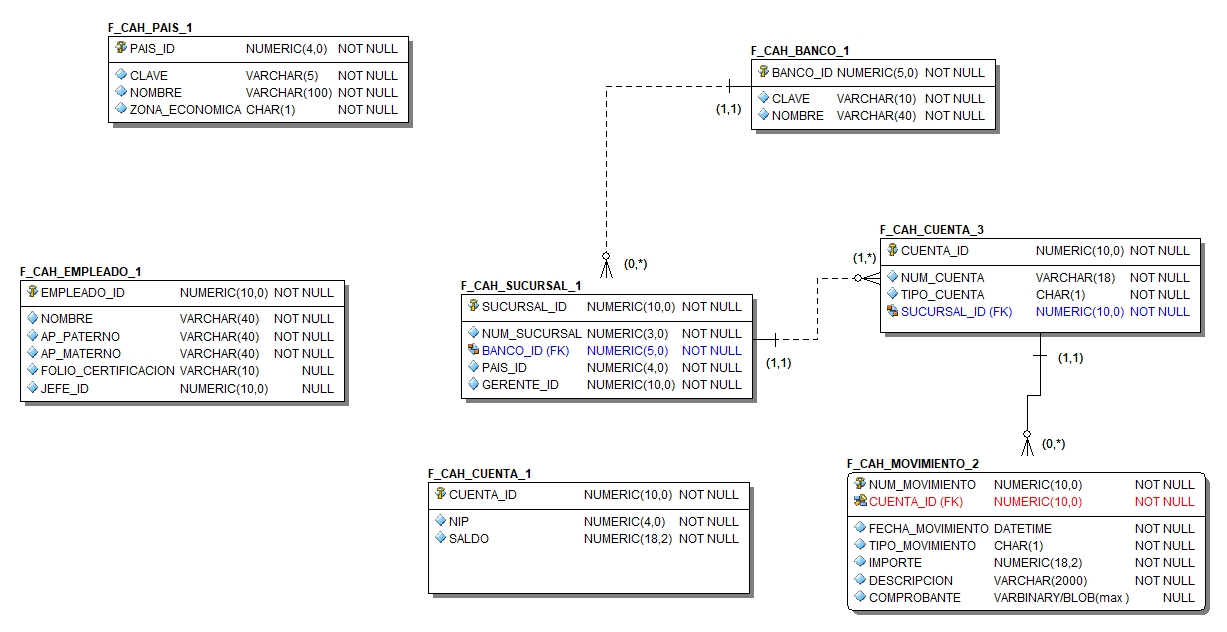
\includegraphics[scale=0.5]{images/P4_N1.jpg}
    
    \newpage
    {\LARGE Sitio N2 \par}
    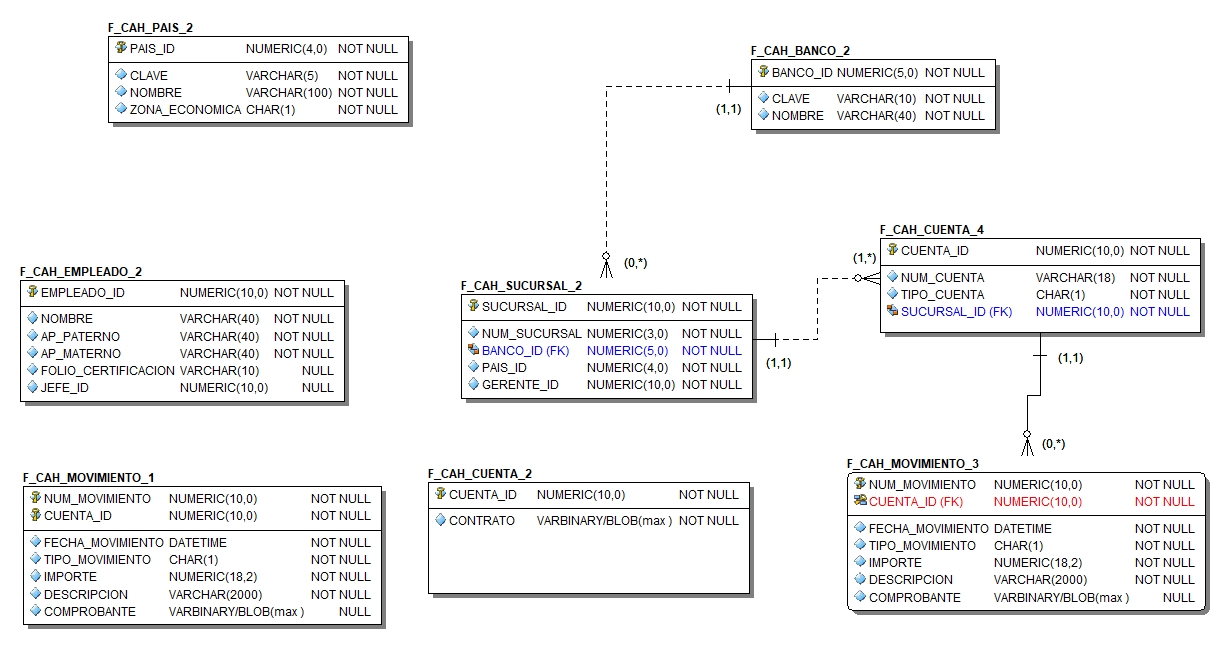
\includegraphics[scale=0.5]{images/P4_N2.jpg}

    \end{landscape}

    \newpage
    
    \section{Conclusiones}
    Hicimos uso de la teoría vista en clase para realizar una fragmentación de tablas sobre un caso de estudio, analizamos que tipo de fragmentación íbamos a realizar, para el caso de la horizontal primaria, saber cuál era la condición de selección, la derivada saber respecto a qué tabla tenemos que fragmentar y para el vertical cuales son las columnas que debemos fragmentar. Una vez definidos los fragmentos se analizó cuales son las restricciones de referencia que debíamos dejar, sabiendo que sólo se conservan aquellas donde se aplicó una fragmentación horizontal derivada, es aquí dónde se presentó la mayor complejidad de la práctica. Lo anterior ayudó a llevar la teoría a la práctica, ya que se diseñaron los modelos relacionales de los sitios, con sus respectivos fragmentos. La práctica sirvió para reflexionar que debemos colocar los fragmentos de acuerdo a las reglas de negocio, por ejemplo, colocamos fragmentos el sitio N2 por el hecho de que tenía altas capacidades de almacenamiento. 
    
    \begin{thebibliography}{1}
\bibitem{ORACLE} \url{https://www.techonthenet.com/oracle/datatypes.php}
\end{thebibliography}
\end{document}
